\documentclass[10pt]{beamer}

\usetheme{CambridgeUS}
\usepackage[english, russian]{babel}
\usepackage[utf8]{inputenc}
\usepackage{caption}
\usepackage{etoolbox}
\usepackage{multicol}
\usepackage{listings}
\usepackage{color}

\definecolor{mygreen}{rgb}{0,0.6,0}
\lstset{
  basicstyle=\ttfamily\footnotesize,        % the size of the fonts that are used for the code
  breaklines=true,                 % automatic line breaking only at whitespace
  captionpos=b,                    % sets the caption-position to bottom
  commentstyle=\color{mygreen},    % comment style
  keywordstyle=\color{blue},       % keyword style
  stringstyle=\color{red},     % string literal style
  showstringspaces=false,
  morekeywords={include, printf},
  texcl=true     %<---- added
  numbersep=14pt
}

\title[\href{https://goo.gl/NRgp8K}{https://goo.gl/NRgp8K} (Term 3)]{Умные указатели}
\author[Зацепин Михаил]{Зацепин Михаил}
\institute[МФТИ] 
{Московский физико-технический институт\\*}
\date{Москва, 2018}
\subject{Computer Science}

\begin{document}

\begin{frame}
  \titlepage
\end{frame}

\begin{frame}{Содержание}
\begin{multicols}{2}
\tableofcontents
\end{multicols}
\end{frame}

\section{raw pointers}
\begin{frame}{Чем нас не устраивают обычные указатели (raw pointers)}
\begin{itemize}
\item{Нельзя понять, является ли указатель \textcolor{red}{владеющим}}
\item{\textcolor{red}{Каким образом} нужно  \textcolor{red}{уничтожить} то, на что указывает указатель}
\item{Нужно уничтожить \textcolor{red}{ровно один} раз}
\item{Как понять, является ли указатель \textcolor{red}{висячим}, т.е. что он указывает на память, которая больше не хранит объект}
\end{itemize}
\end{frame}

\section{smart pointers}
\begin{frame}{Умные указатели в C\texttt{++}}
\begin{itemize}
\item{\texttt{auto\_ptr} (\textcolor{red}{deprecated} в C\texttt{++}11, \textcolor{red}{removed} в C\texttt{++}17)}
\item{\texttt{unique\_ptr}}
\item{\texttt{shared\_ptr}}
\item{\texttt{weak\_ptr}}
\end{itemize}
\end{frame}

\section{\texttt{unique\_ptr}}
\begin{frame}[fragile]{\texttt{unique\_ptr}}
\begin{lstlisting}[language=C++]    
    template<class T, class Deleter> class unique_ptr;
\end{lstlisting}

\begin{enumerate}
    \item Владеет объектом, на который указывает.
    \item Запрещает копирование, но разрешает перемещение (move). 
    \item При уничтожении указателя, уничтожается и объект, которым он владеет. 
    \item Позволяет возвращать из функции объекты, выделенные на динамической памяти.
    \item Кроме того корректно уничтожает такие объекты при раскрутке стека во время проталкивания исключений.
    \item Преобразуется в \texttt{shared\_ptr}
\end{enumerate}
\end{frame}

\section{\texttt{shared\_ptr}}
\begin{frame}[fragile]{\texttt{shared\_ptr}}
\begin{lstlisting}[language=C++]
    template<class T> class shared_ptr;
\end{lstlisting}

\begin{enumerate}
    \item \textcolor{red}{Совместное} владение.
    \item Реализация - \textcolor{red}{счетчик ссылок}:
    \begin{enumerate}
        \item Создание \texttt{shared\_ptr} - увеличение счетчика ссылок на 1
        \item Разрушение \texttt{shared\_ptr} - уменьшение счетчика ссылок на 1
        \item Счетчик становится равным 0 - разрушение объекта
    \end{enumerate}
    \item \texttt{deleter} также присутствует, но не как часть типа, а как часть \textcolor{red}{управляющего блока}
\end{enumerate}
\end{frame}

\section{Управляющий блок \texttt{shared\_ptr}}
\begin{frame}[fragile]{Управляющий блок \texttt{shared\_ptr}}
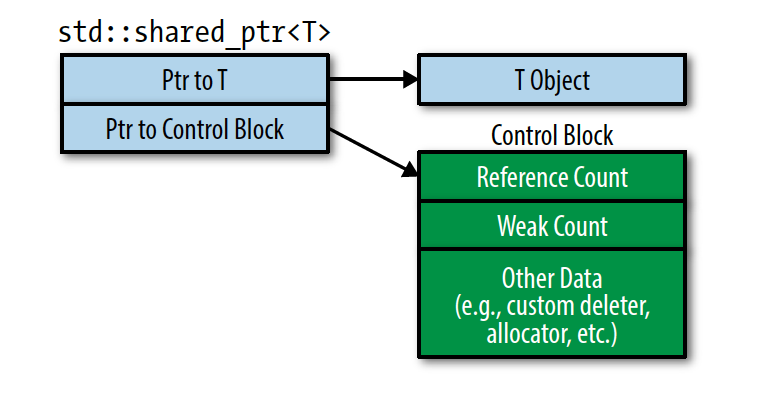
\includegraphics[scale=0.75]{Term_3/Source/Pictures/shared.png}
\end{frame}

\section{Особенности использования \texttt{shared\_ptr}}
\begin{frame}[fragile]{Особенности использования \texttt{shared\_ptr}}
\begin{lstlisting}[language=C++]
    int* ptr = new int(10);
    std::shared_ptr<int> smart_ptr1(ptr);
    std::shared_ptr<int> smart_ptr2(ptr);
\end{lstlisting}
\pause
\textcolor{red}{Неправильно: два счетчика ссылок}

\pause

Корректно:
\begin{lstlisting}[language=C++]
    std::shared_ptr<int> smart_ptr1(new int(10));
    std::shared_ptr<int> smart_ptr2(smart_ptr1); 
\end{lstlisting}
\end{frame}

\section{Производительность \texttt{shared\_ptr}}
\begin{frame}[fragile]{Производительность \texttt{shared\_ptr}}
\begin{enumerate}
    \item Размер х2 по сравнению с raw\texttt{-}указателем
    \item Динамическое выделение памяти под управляющий блок
    \item Атомарный инкремент / декремент
\end{enumerate}
\end{frame}

\section{\texttt{weak\_ptr}}
\begin{frame}[fragile]{\texttt{weak\_ptr}}
\begin{lstlisting}[language=C++]
    template<class T> class weak_ptr;
\end{lstlisting}

\begin{enumerate}
    \item Невладеющий ''напарник'' \texttt{shared\_ptr}
    \item Отслеживание висячих объектов
    \item Отсутствует operator*() и операторы сравнения
\end{enumerate}

\end{frame}

\section{\texttt{Использование weak\_ptr}}
\begin{frame}[fragile]{Использование \texttt{weak\_ptr}}
\begin{lstlisting}[language=C++]
    std::shared_ptr<int> shared_ptr(new int(10));

    // Создание из weak\_ptr или shared\_ptr
    std::weak_ptr<int> weak_ptr(shared_ptr);

    // Получение доступа. Два способа:
    std::shared_ptr<int> new_shared_ptr = weak_ptr.lock();
    std::shared_ptr<int> new_shared_ptr_2(weak_ptr);

\end{lstlisting}

В чем разница между двумя способами получения доступа?

\pause
Поведение в случае если weak\_ptr висячий:
\begin{enumerate}
    \item \texttt{lock} - вернет нулевой указатель
    \item конструктор бросит исключение \texttt{bad\_weak\_ptr}
\end{enumerate}
\end{frame}

\section{\texttt{Применение weak\_ptr}}
\begin{frame}[fragile]{Применение \texttt{weak\_ptr}}
\begin{enumerate}
    \item Кеширование объектов
    \item Решение проблемы циклических ссылок
\end{enumerate}
\end{frame}

\section{\texttt{make\_unique} и \texttt{make\_shared} vs \texttt{new}}
\begin{frame}[fragile]{\texttt{make\_unique} и \texttt{make\_shared} vs \texttt{new}}
\begin{enumerate}
    \item Краткость кода
    \item Повышение безопасности кода
    \item Повышение производительности
    \pause
    \item \textcolor{red}{Но не всегда}
\end{enumerate}
\end{frame}

\section{\texttt{Использование \texttt{make\_unique} и\texttt{make\_shared}}}
\begin{frame}[fragile]{Использование \texttt{make\_unique} и \texttt{make\_shared}}
\begin{lstlisting}[language=C++]
    // Сравните
    std::unique_ptr<Task> ptr(new Task);
    auto ptr2(std::make_unique<Task>());

    // А вдруг исключение?
    processTask(std::unique_ptr<Task>(new Task), 
                computeNewTaskPriority());
\end{lstlisting}
\end{frame}

\section{Литература}
\begin{frame}[fragile]{Литература}
\begin{enumerate}
    \item Скотт Мейерс. Эффективный и современный C++
    \item Скотт Мейерс. 55 способов ... 
\end{enumerate}
\end{frame}

\end{document}
